\documentclass[../all.tex]{subfiles}
\begin{document}
%%%%%%%%%%%%%%%%%%%%%%%%%
\section{Experimentación} % Evaluación
%%%%%%%%%%%%%%%%%%%%%%%%%
	Una vez explicadas las tecnologías usadas y el marco del trabajo, se procederá a explicar detalladamente como se ha llegado a la resolución del trabajo detallando los procedimientos seguidos y justificando la elección de las librerías, algoritmos y técnicas usadas junto a los resultados obtenidos en cada una de las fases del proyecto.  El proyecto se divide en 4 fases donde todas son dependientes de la fase 0 y la fase 3 de las tres anteriores.  La 1 y 2 no dependen entre si dado que son algoritmos que buscan cosas diferentes, pero sí que necesitan toda la información extraída en la fase 0 para analizarla y enviar los resultados a la fase 3 donde se trataran y se decidirá si ese tweet contiene o no una mentira.
	
\subsection{Problemática lenguaje natural}
	El procesamiento del lenguaje natural (PLN o NLP en sus siglas anglosajonas) es una rama de la Inteligencia Artificial encargada de estudiar métodos de comunicación entre máquina y hombre a través del lenguaje natural, es decir, el lenguaje empleado de forma habitual en una conversación escrita u oral entre personas.\\ 
	
	El lenguaje natural presenta muchas características que lo hacen un verdadero reto para las ciencias de la computación. Como suele pasar en el mundo de la Inteligencia Artificial, una tarea que puede parecer para una máquina. Aspectos como la ambigüedad, la espontaneidad, la falta de fluidez, las referencias y las abreviaturas son difíciles de procesar.

\subsubsection{Homonimia}
	La homonimia  es la cualidad de dos palabras, de distinto origen y significado por evolución histórica, que tienen la misma forma, es decir, la misma pronunciación o la misma escritura\cite{HomonimiaPolisemia}.\\
	
	Un ejemplo estaría en la palabra \textbf{vela}:
	\begin{enumerate}[resume]
		\setcounter{enumi}{0}
		\item Acción de velar; cilindro de cera con una mecha para iluminar. (Ambos sentidos relacionados con el verbo velar.
		\item Tela grande que aprovecha la fuerza del viento, especialmente en un barco.
	\end{enumerate}

	En castellano de homonimias tenemos diferentes clases:
	
	\begin{enumerate}[resume]
		\setcounter{enumi}{0}
		\item \textbf{Homónimos lexicales}: los que pertenecen a la misma categoría gramatical: onda y honda, botar y votar, haya y aya, ojear y hojear.
		\item \textbf{Homónimos gramaticales}: los que no pertenecen a la misma categoría gramatical: cabe verbo y cabe preposición, o los que perteneciendo a la misma categoría gramatical se diferencian en alguna marca morfemática: el pez, la pez; el orden, la orden.
		\item \textbf{Homónimos léxico-gramaticales}: los que se han formado a través de un cambio de funciones: poder (verbo) poder (sustantivo)
		\item \textbf{Homónimos morfológicos}: cuando se producen diferentes formas de una sola palabra: decía primera y tercera personas del pretérito imperfecto de indicativo; o se dan formas correspondientes de palabras diferentes: fui (de ser e ir); ve (de ir y de ver), etc.
	\end{enumerate}

\subsubsection{Polisemia}
	La polisemia, en lingüística, se presenta cuando una misma palabra o signo lingüístico tiene varias acepciones o significados. Una palabra polisémica es aquella que tiene dos o más significados que se relacionan entre sí\cite{HomonimiaPolisemia}.\\
	
	Cabe resaltar que la polisemia puede surgir por diversos motivos. Por un lado, el vocabulario figurado produce polisemia por medio de las metáforas y las metonimias. Por ejemplo: los brazos de un río, las patas de una mesa. La especialización y el lenguaje técnico también atribuyen un significado específico a ciertos términos (como en el caso del ratón en la informática).\\
	
	La influencia extranjera y las modificaciones de aplicación son otras condiciones que favorecen la polisemia: una muestra de esto es el vocablo botón que nació con la indumentaria y luego pasó a utilizarse también en los artefactos electrónicos.\\
	
	Un ejemplo estaría en la palabra \textbf{cabo}:
	\begin{enumerate}[resume]
		\setcounter{enumi}{0}
		\item (masculino) Punta de tierra que penetra en el mar.
		\item (masculino/femenino) Escalafón militar.
		\item (masculino) Cuerda en jerga náutica.
	\end{enumerate}
\newpage
\subsubsection{Anáfora y elipses}
	La anáfora se puede definir como la palabra o palabras que asumen el significado de una parte del discurso (texto) que ya se ha mencionado antes\cite{AnaforaElipses}.\\
	
	Un ejemplo de anáfora sería:
	\begin{itemize}[resume]
		\item Estoy de paso por Madrid. {\small(Madrid)} Es maravillosa. 
	\end{itemize}
	Cuando el elemento sustituido aparece después del sustituto, hablamos de catáfora.\\
	Un ejemplo de catáfora sería:
	\begin{itemize}[resume]
		\item Quería estar con \underline{Jesús}; pero no \underline{lo} he visto en toda la tarde. 
	\end{itemize}

	Por otro lado tenemos las elipses que es la omisión o supresión de una o varias palabras que ya se habían mencionado antes o que se pueden presuponer o sobreentender. Esta construcción evita el uso de repeticiones innecesarias.\\
	Un ejemplo de elipse sería:
	\begin{itemize}[resume]
		\item El concierto fue genial, la comida {\small(fue)} regular. 
	\end{itemize}
\subsubsection{Sintaxis no normalizada}
	 Otro problema que nos plantea el análisis de lenguaje natural es el hecho de que su estructura no está normalizada, es decir, a la hora de utilizar el lenguaje en español, no se utiliza una sintaxis concreta y bien definida, si no que a la hora de expresar una misma idea, ésta se puede estructurar de diversas maneras.
 	\begin{itemize}[resume]
	 	\item Me encantan las mañanas de domingo.
	 	\item Las mañanas de domingo me encantan.
 	\end{itemize}
	 Ambas oraciones expresan la misma idea utilizando un orden diferente en las distintas palabras que las componen.
\newpage
\subsubsection{Contexto}
	El contexto es el conjunto de circunstancias (materiales o abstractas) que se producen alrededor de un hecho, o evento dado, que hacen que una palabra pueda tomar varios sentidos según el momento en el cual se utiliza.\\
	
	Un claro ejemplo de la importancia del contexto es la ironía, a un suceso malo se puede contestar con otra frase 'mala' como sería el caso de; \textit{¡Otra vez no!}, con una frase buena del estilo; \textit{¡Qué bien!} donde estaríamos siendo irónicos o con una frase como; \textit{¿Porqué a mí?}.
	
\subsubsection{Otras circunstancias}

	Aparte de toda esta serie de fenómenos que se dan en la lengua formal, hay que tener que cuenta otros aspectos que se dan en ambientes más coloquiales como son las redes sociales.\\
	
	En la siguiente tabla se muestran algunos ejemplos de cómo un mismo mensaje puede tener formas diferentes según el usuario y el medio en el que lo escriba.
	\begin{center}
		\begin{tabular}{ | m{7cm}| m{7cm} | } 
			\hline
			\textbf{Texto de ejemplo} & \textbf{Explicación}\\ 
			\hline
			Messi es el mejor jugador de la historia del fútbol. & Frase correcta \\ 
			\hline
			Mesi es el mejor jugador de la istoria del futbol; & Faltas de ortografía\\ 
			\hline
			MesSi es el MeJor juGAdor de la hIStoriA del fúTBol :) & Incluir mayúsculas y símbolos innecesarios\\ 
			\hline
			Messiiii es el mejor jugador de la historia del futbooooool & Añadir repetición de letras para darle mayor énfasis a la palabra\\ 
			\hline
			Mssi s l mjor jugadr d la histria dl futbol  & Lenguaje SMS.\\ 
			\hline
			¡Vamos equipo! & Brevedad y ambigüedad del texto \\ 
			\hline
		\end{tabular}
	\end{center}

\newpage
\subsection{Fase 0 - Extracción de la información}
	
	Esta es la fase cero es donde se diseña el proyecto y por eso es la fase que más veces ha tenido que ser modificada para ajustarse a las necesidades reales del proyecto descubiertas en las siguientes fases a lo largo de la implementación de estas. No se llama fase cero solo porque los informáticos estamos acostumbrados a contar desde cero, sino que también no solo es una fase previa de almacenar datos en el proyecto, sino que a lo largo que ha ido evolucionando el proyecto se ha tenido que ir modificando código y estructuras alocadas en esta fase. Podríamos decir que a parte de una fase previa también es una fase paralela a todo el proyecto.\\
	
	Antes de nada lo que se decidió es que dada la acotación que se hizo de solo buscar trolls en el ámbito de los deportes este proyecto sea fácilmente escalable así que se creó una clase \textit{Utils} con clases para definir los temas por variables como nombre, lista de palabras, id, etc y otra clase donde se hace una relación de un id numérico creciente con el nombre del tema así pues, todos los algoritmos tienen un bucle y solo tienen que buscar por cada uno de los id’s sin necesidad de modificar nada del código únicamente se necesita incluir el nuevo tema con su id correspondiente en esa clase. Esto permite añadir una capa de abstracción de los temas que hay a los algoritmos y diccionarios dado que tanto los algoritmos como los diccionarios utilizan esa lista de temas sin saber cuántos hay por lo tanto si añades un nuevo tema sin darse cuenta llenara el diccionario con ese nuevo tema y clasificara el texto con ese tema si ese tweet trata sobre ese nuevo tema.\\
	
	 A continuación se puede ver como es la función para obtener los deportes que se buscaran y que por su estructura tiene un muy fácil crecimiento de los temas:

	\begin{figure}[H]
		\centering
		\includegraphics[height=10cm, width=10cm]{imgs/UtilsScale.png}
		\caption{Función que devuelve el id o el nombre del tipo en esa posición.}
	\end{figure}

	La primera tarea en esta fase es la de guardar los diccionarios que no son más que una ontología propia y montar toda la base de datos en MongoDB dado que sin ellos no se puede hacer nada. Se decidió que la base de datos fuese en Mongo dado que es la idónea para guardar grandes cantidades de textos por su indexación. En esta base de datos se encuentran tweets de ejemplo, un diccionario con palabras que no aportan significado a las frases como es el caso de los artículos, un diccionario para cada deporte donde se encuentran palabras primarias, secundarias y excluyentes y por último un diccionario con palabras que relacionan directamente a cada uno de los sentimientos. En los apartados siguientes de experimentación en la fase uno y dos se explicará para que sirve cada uno de los diccionarios, en esta fase solo se usa el de palabras vacías.\\
	
	\begin{figure}[H]
		\centering
		\includegraphics[height=14cm, width=16cm]{imgs/MongoDB_DBS.png}
		\caption{Base de datos del proyecto.}
	\end{figure}

	Solo recordar que este es el estado final de la base de datos a la cual se le han ido añadiendo campos y clases según se han necesitado. El primer diccionario que se creo fue el de las palabras vacías para poder excluir todas aquellas palabras que no nos aportaban nada y así tener unos mejores resultados. La primera opción fue buscar cada uno de los deportes en Wikipedia con una conexión a través de Python y de ese texto obtenido eliminar preposiciones, artículos y demás palabras encontradas en el fichero y guardar el número de repeticiones de cada una de las palabras que se encontraban en ese fichero de palabras vacías. Con esto conseguimos tener una lista de todas las palabras que se encuentran en Wikipedia sobre cada uno de los deportes y el número de veces que aparece. A partir de este primero diccionario se fue trabajando en paralelo creando algoritmos y afinando un diccionario propio más preciso donde se busco por Internet vocabulario de cada uno de los deportes, así como sus personas, equipos y campeonatos más relevantes. Con el diccionario de Wikipedia se tenían unos resultados algo pobres en las siguientes fases que se vieron mejorados gracias al diccionario escrito a mano. La diferencia principal a parte de que en Wikipedia no están todas las palabras de un deporte es que en Wikipedia solo almacenábamos las palabras más repetidas y el porcentaje con el que aparecían y con el diccionario propio conseguimos hilar más fino gracias a tener palabras principales que definen en el deporte, palabras secundarias que son las que se usarían en la jerga de ese deporte y palabras excluyentes que no se dirían nunca en ese deporte.\\
	
	\begin{figure}[H]
		\centering
		\includegraphics[height=14cm, width=16cm]{imgs/DBSportsWikipedia.png}
		\caption{Diccionario de los deportes guardados obtenidos por Wikipedia.}
	\end{figure}
	\begin{figure}[H]
		\centering
		\includegraphics[height=14cm, width=16cm]{imgs/DBSports.png}
		\caption{Diccionario de los deportes propio.}
	\end{figure}

	\begin{figure}[H]
		\centering
		\includegraphics[height=14cm, width=14cm]{imgs/DBSentiments.png}
		\caption{Diccionario de los sentimientos propio.}
	\end{figure}

	Una vez obtenido el diccionario de los deportes tocaba ponerlo en práctica para ver cómo funcionaba así que se probaron frases escritas a mano y cuando empezamos a comprobar que los algoritmos funcionaban se probó la conexión que habíamos hecho previamente a Twitter con la librería Tweepy que proporciona una API muy sencilla para obtener información sobre usuarios, así como sus tweets y hacer búsquedas por hashtags. Estos tweets fueron almacenados en MongoDB con la finalidad de comprobar siempre los algoritmos con los mismos tweet dado que un estudio de \textit{Designly}. \footnote{\url{https://www.infobae.com/2013/08/07/1500503-cuantos-tuits-se-escriben-segundo-el-mundo/}} dice que se escriben 3.935 tweets cada segundo así que nuestros resultados variaban en cada ejecución.\\
	
	Una vez están las conexiones con MongoDB y Twitter creadas y se tiene toda la información guardada se vio que las consultas en las siguientes fases se hacían de forma lenta así que para mejorar tiempos de consulta se decidió guardar los diccionarios en un AVL Tree. \\
	
	\begin{figure}[H]
		\centering
		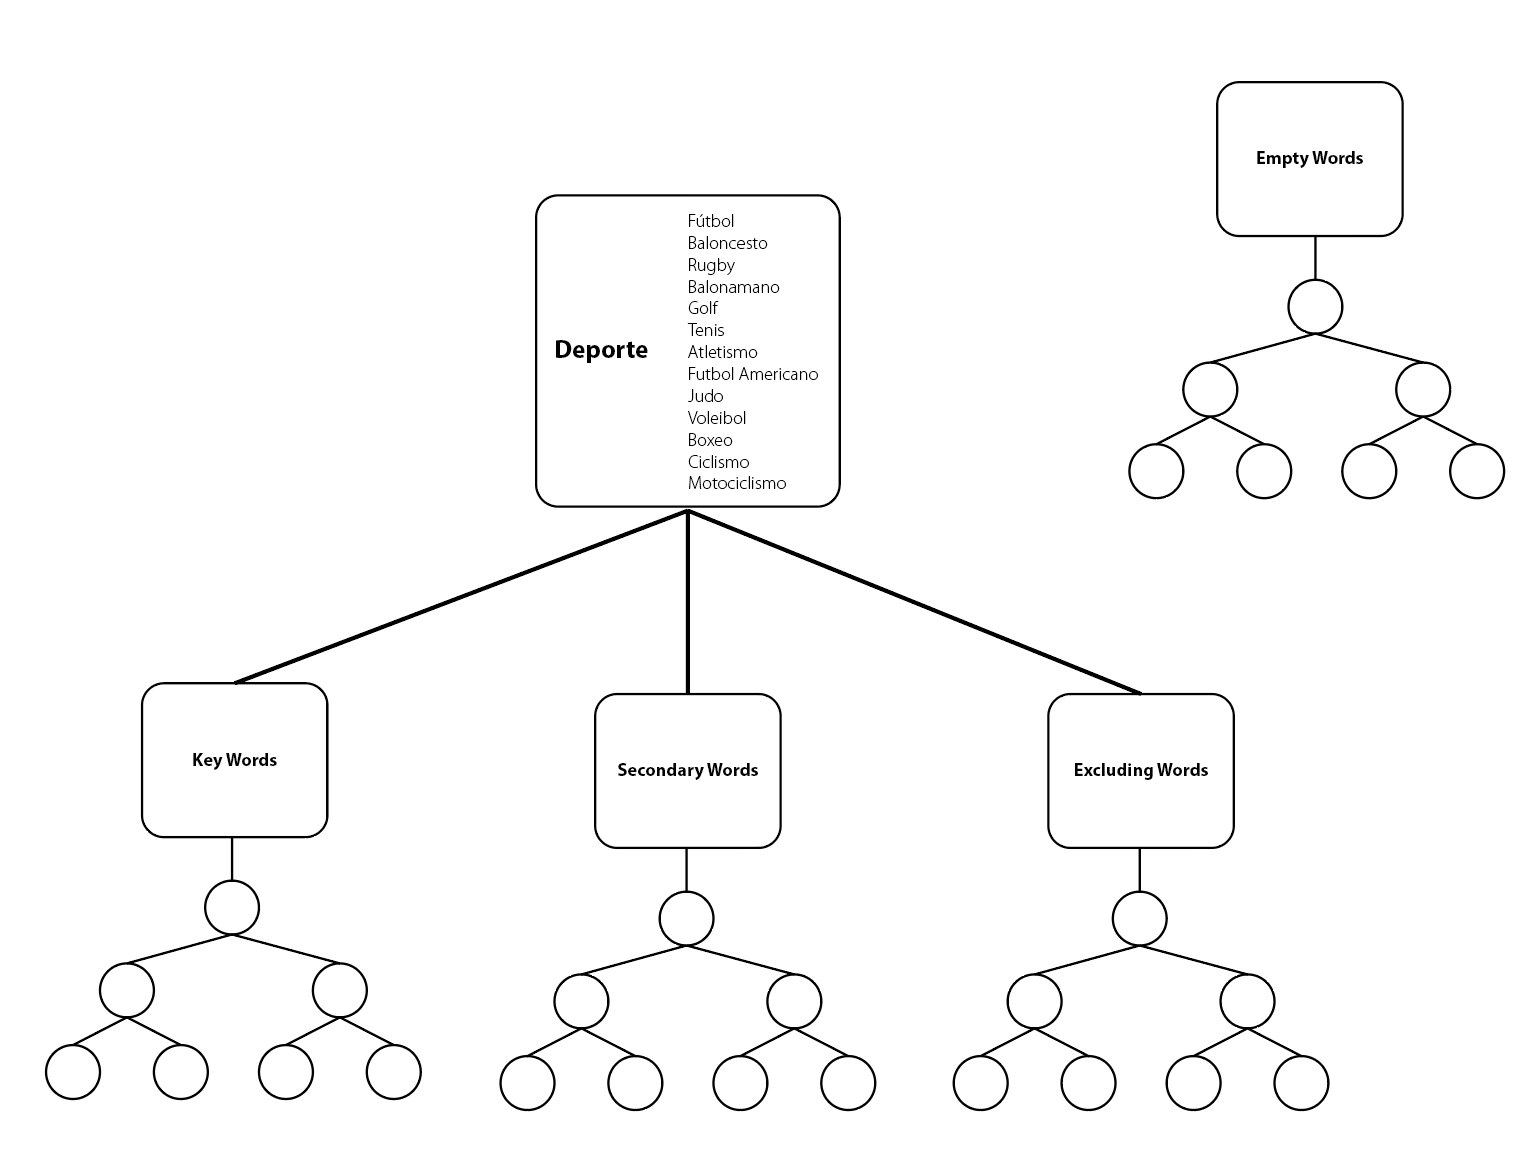
\includegraphics[height=14cm, width=14cm]{imgs/treeScheme.png}
		\caption{Esquema estructuración de los datos}
	\end{figure}

	\newpage
	Una vez el árbol esta creado y se tiene almacenado en él los diccionarios pertinentes se procede a tratar el tweet que se quiere analizar o en su defecto el texto introducido por el usuario.  Cada tweet lo replicamos y guardamos el tweet original, aplicándole el \textit{stemmer} para obtener la raíz de cada palabra y una ultima con el tweet sin las palabras vacías, todas las palabras separadas y en forma de \textit{array}. Una vez teniendo el tweet original y sus variaciones se enviaran estas a las posteriores fases para analizarlas. Se quiso conservar en todo momento el texto original por si se necesitaba en algún algoritmo. El único problema que hubo con la librería de Tweepy es que solo proporciona tweets de cien en cien así que se tenía que ir guardando la fecha del último tweet y hacer peticiones siempre a partir de esa fecha hasta que tengamos el número de tweets que se querían.\\
	
	Este análisis se aplica no solo al tweet a analizar sino que también recoge los últimos veinte tweets del usuario y si hizo algún retweet o mención se analizan los últimos diez tweets de ese otro usuario para tener un análisis más fiable, eso sí, se para en el segundo nivel, es decir solo se mira el usuario del retweet y como mucho si ese perfil tenía otro retweet se estudia ese usuario y no se adentrará a más perfiles.\\
	
	A continuación, podemos observar dos ejemplos de como tratan los tweets y por lo tanto, de como reciben los textos las siguientes fases.\\
	
	\begin{figure}[H]
		\centering
		\includegraphics[height=15cm, width=16cm]{imgs/EXStemmed.png}
		\caption{Ejemplo de salida de la frase una vez tratada.}
	\end{figure}
	\newpage
	En la siguiente figura se pueden ver las clases implementadas más importantes:
	\begin{figure}[H]
		\centering
		\includegraphics[height=15cm, width=15cm]{imgs/MyClass.png}
		\caption{Clases propias más importantes.}
	\end{figure}

	En conclusión, es la encargada de crear y gestionar conexiones con MongoDB y Twitter así como de almacenar los datos obtenidos en esas conexionas y enviarlas a las siguientes fases para su posterior tratamiento. 


\newpage
\subsection{Fase 1 - Clasificación de texto según temática}

	La tarea de esta fase es la de analizar cada uno de los tweets y decir cada uno de que tema hace referencia para finalmente saber sobre que \textit{X} temas habla ese usuario donde \textit{X} esta fijada en tres aunque en los ejemplos que se mostraran para hacerlo más claro solo se dice el tema sobre el que más habla. \\
	
	Recordad que los temas sobre los que se centra el algoritmo son de los que hicimos diccionario:\\
	
	 \begin{enumerate}
	\begin{multicols}{2}
		\setcounter{enumi}{-1}
		\item Fútbol.
		\item Baloncesto.
		\item Rugby.
		\item Balonmano.
		\item Golf.
		\item Tenis.
		\item Atletismo
		\item Judo.
		\item Voleibol.
		\item Boxeo.
		\item Ciclismo
		\item Motociclismo.
		\item Fútbol americano
	\end{multicols}
	\end{enumerate}

	En la figura siguiente se muestra un esquema que representa la idea principal del funcionamiento de esta fase.\\
	
	\begin{figure}[H]
	    \centering
	    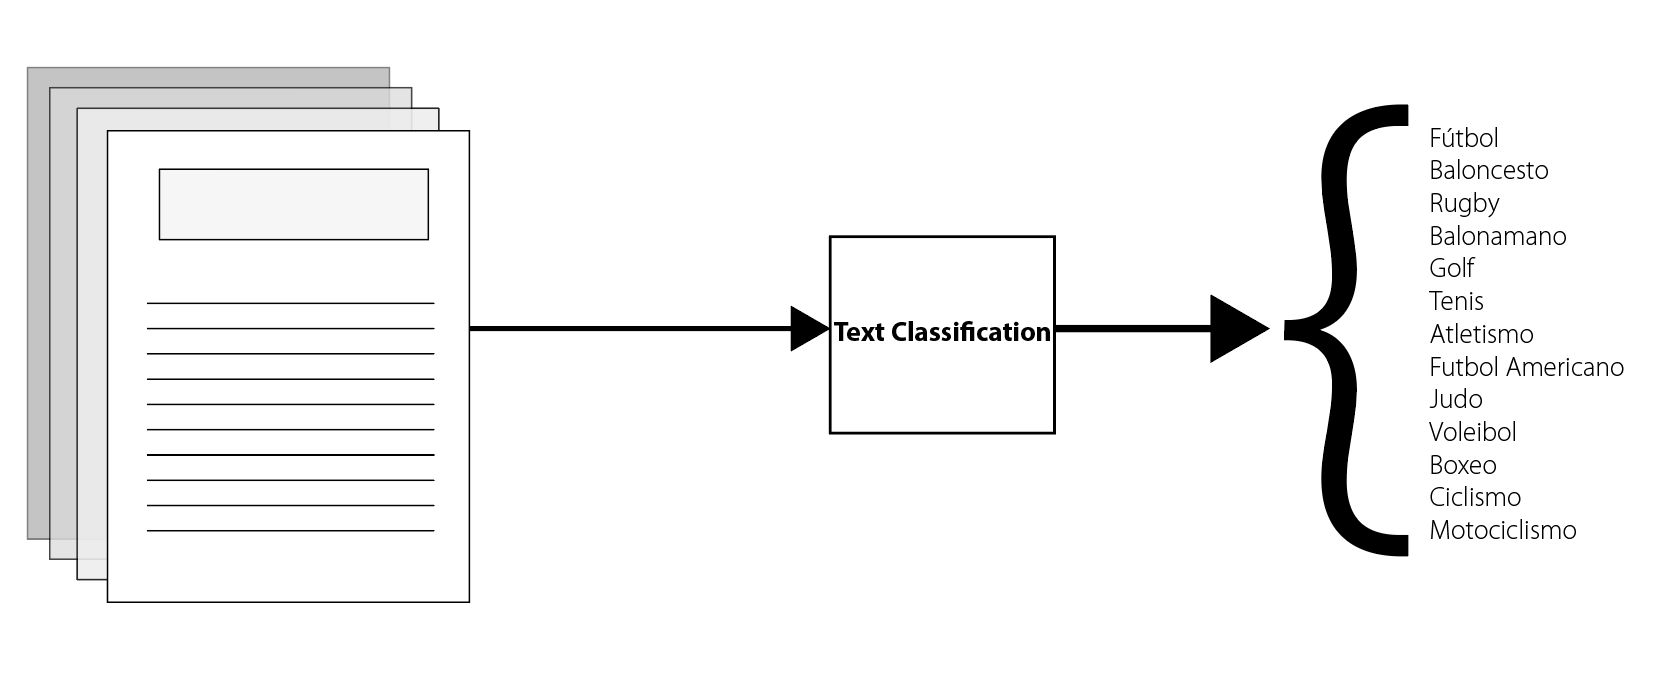
\includegraphics[height=15cm, width=15cm]{imgs/textClassification.png}
	    \caption{Idea principal del clasificador de texto}
	\end{figure}


	Para la clasificación de los Tweets según la temática lo primero que se hizo fue implementar unos algoritmos que se entrenaban mediante el mismo Twitter. Lo que se hizo fue pedirle a la fase cero que nos enviase X tweets donde el 33\% de estos tweets se utilizaban para entrenar el algoritmo. X son el número de tweets totales que se tendrán para hacer las pruebas pero realmente se piden X’ tweets donde X’ corresponde a (X/(Número de Temas)) por lo tanto, en nuestro caso, X’=X/13. Así pues se hicieron pruebas donde X tomaba el valor de: 13, 26, 52, 104, 208, 416, 832, 1.500, 3.000, 5.000 y 10.000.  En el siguiente gráfico podemos observar los resultados de la accuracy de los algoritmos con los valores anteriores.\\
	
	\begin{figure}[H]
		\centering
		\fbox{
			\includegraphics[height=15cm, width=\linewidth]{imgs/TextClassificationAccuracy.png}
		}
		\caption{Resultados obtenidos en clasificación de texto sin diccionario.}
	\end{figure}

	En el diagrama anterior se puede observar como el peor algoritmo es el SVM dado que nunca se puede obtener un accuracy mayor al 0,1. Esto viene dado a que  tiene una gran demanda de buenos tokenizadores (filtros) pero, el diccionario del conjunto de datos siempre tiene tokens sucios o ruido porque son los tweets de otros usuarios, este funcionaria mejor si se aplicará el diccionario creado ya que ese diccionario contiene palabras que definen cada deporte por separado y no verbos o adjetivos que se pueden usar indistintamente en cada uno de los deportes. También se puede apreciar que todos los algoritmos coinciden en que, por un juego de datos menor a 1000 twets, ninguno obtiene un accuracy mayor al 0,5.  Los algoritmos que obtienen mejor accuracy con menos de 1500 tweets es XGBoost y y a partir de los 2000 tweets los que devuelven mejor accuracy es Random Forest Model acercándose al 0,9 a partir de los 5000 tweets donde de estos 5000 solo 1560 se están utilizando para entrenar el algoritmo.\\
	
	Los resultados anteriores se podrían dar por satisfactorios y acabar la investigación, pero primero habría que analizarlos más detalladamente y darse cuenta de que tienen algo de trampa.  Los resultados dados así son muy gratificantes, solamente descargas 2000 tweets y obtienes un accuracy del 0,8 donde cualquier analista te lo compraría y daría por cerrado el proyecto. Bien, no todo es tan fácil, descargarse 2000 tweets es más difícil de lo que parece dado que la API que proporciona Twitter para Python solo devuelve un máximo de 100 tweets por petición, es decir, para pedir 2000 tweets hay que hacer 20 consultas las cuales no son rápidas y tiene que obtener la fecha del tweet número cien para en la siguiente petición pedir tweets a partir de esa fecha y así hasta que logres alcanzar los 2000 tweets. Esto tampoco parece un gran problema, en una media de 10 segundos consigues los tweets que quieres, pero si a esto le sumas que solo puede hacer 100 peticiones cada media hora, tienes el resultado que cada 30 minutos solo puedes ejecutar tu algoritmo cinco veces.\\
	
	Otro problema que se presenta es la proximidad temporal de los tweets. Esto se refiere a que cogemos los últimos tweets que se han escrito en Twitter y los usuarios normalmente comentan las últimas novedades y lo sucedido en las últimas horas y esto es una ventaja dado que usualmente compararemos tweets parecidos al del usuario, pero también puede pasar que un usuario hablé sobre lo que paso ayer u otro día anterior y al hacer la búsqueda con estos algoritmos ninguno se parezca y lo clasifiquemos de forma errónea.\\
	
	Para solucionar estos problemas más las restricciones de tiempos de los algoritmos se decidió utilizar Naive Bayes con un dataset de 700 tweets donde se consigue un accuracy del 0,4-0.5 y es el más rápido en cuanto a tiempo se refiere gracias a la sencillez del algoritmo. Con los resultados obtenidos se hace una media de que deporte puede tratarse entre los dos algoritmos y se acaba de afinar con un tercer algoritmo el cual es propio y se ejecuta mediante un diccionario también propio. \\
	
	{\color{red} 
		TODO:    MATRIZ DE CONFUSION NAIVE BAYES CON 700
	}
	\newpage
	Este diccionario de cada deporte esta almacenado en un árbol AVL Tree el cual es una estructura de datos ordenada y los costes temporales de búsqueda son O (log(n)). Otra ventaja que tiene este árbol es el poder clasificar por palabras compuestas, es decir que por ejemplo si buscas la falta de baloncesto 'campo atrás', gracias a la búsqueda que se ha implementado en este árbol, se encontrará. En la siguiente figura se puede observar que se tarda 1,32 segundos en tratar sin el árbol y 0,33 analizando con el árbol AVL implementado.\\
	
	\begin{figure}[H]
		\centering
		\includegraphics[height=15cm, width=15cm]{imgs/ComparacionAVL.png}
		\caption{Comparativa entre guardar diccionario en una \textit{array} o en un árbol AVL.}
	\end{figure}
	
	Una vez este algoritmo recibe el tweet previamente tratado en la fase 0, es decir que tengo el tweet separado por palabras y sin artículos ni preposiciones, actuará el algoritmo. Este algoritmo principalmente lo que hace es buscar apariciones de las palabras del tweet en los arboles creados, uno por cada deporte y además uno que contiene palabras primarias las cuales si se encuentra sumara 1 punto a ese deporte, palabras secundarias las cuales si las encuentra sumara 0,25 puntos sobre ese deporte y palabras excluyentes las cuales si se encuentran se restaran 1,5 puntos en ese deporte. Una vez ya no hay más palabras obtenemos los dos deportes con mayor puntuación y se contrastan con los obtenidos en la evaluación anterior del algoritmo Naive Bayes y .\\
	
	\newpage
	En la siguiente figura se pueden observar cuatro ejemplos de como actúa este algoritmo descrito anteriormente que hace uso de los diccionarios de cada uno de los deportes.
	
	\begin{figure}[H]
		\centering
		\includegraphics[height=18cm, width=15cm]{imgs/DictionaryExample.png}
		\caption{Ejemplos de ejecución del algoritmo por diccionario almacenado en un árbol AVL en análisis por temática.}
	\end{figure}

	\newpage
	También se hicieron pruebas con el algoritmo de Naive Bayes entrenándolo, no solo con tweets, sino que también con las palabras que se encontraban en el diccionario como palabras primarias. Esto mejoro los resultados respecto a entrenarlo solo con tweets, pero no a los resultados obtenidos con el diccionario anterior. Por último, se intentó entrenarlo también con las palabras secundarias pero los resultados fueron parecidos.\\
	
	Debido al uso del castellano como lenguaje a analizar todos los análisis se han complicado, un ejemplo de ello es el intentar de utilizar un \textit{stemmer} para obtener la raíces de las palabras ya que, en castellano, es un proceso muy complicado por la riqueza del mismo. En la siguiente figura se puede observar un ejemplo de este problema dónde confunde la preposición para que coge como raíz 'par' con el verbo parar dado que en el diccionario de balonmano y fútbol hay la palabra parada y la define también con la raíz 'par'.\\
	
	 \begin{figure}[H]
	 	\centering
	 	\includegraphics[height=14cm, width=13cm]{imgs/errorStem.png}
	 	\caption{Ejemplos de error en el uso de un \textit{stemmer} en clasificación de texto.}
	 \end{figure}
	
	Para concluir, recordar que se usan los algoritmos NaiveBayes junto al diccionario propio y no solo que estos algoritmos se aplican no solo a un tweet sino, a todos últimos 20 tweets del usuario y los 10 de los perfiles retweeteados si los hay. Una vez hecho esto se envía a la fase tres los resultados y está queda a la espera de tener los resultados de la fase dos.
	
	
\newpage
\subsection{Fase 2 - Análisis del sentimiento}
    El análisis de sentimiento de textos en las redes sociales es el proceso que determina el tono emocional que hay detrás de unas palabras determinadas, si una frase contiene una opinión positiva o negativa sobre un producto, marca, institución, organización, empresa, evento o persona.\\

    Los sentimientos se clasifican en positivos, negativos o neutros. Sin embargo, el lenguaje natural es complejo y ambiguo por lo que enseñar a una máquina a que analice los diferentes matices gramaticales, variaciones culturales, jergas, expresiones coloquiales o a distinguir faltas de ortografía, la sinonimia o la polisemia dentro de un contexto que determina el tono de la conversación es francamente difícil. Así, por ejemplo, ante un comentario sarcástico, la máquina tomaría la frase como algo positivo en vez de algo negativo o expresiones como “LOL, OMG, estuvo geeeeeeeniaaaaaaaal” son dificilísimas de procesar.\\
    
  Como los algoritmos que usaran en esta fase se aplicarán en textos (o tweets) escritos en castellano, los resultados son bastante pobres dado que no se tiene un \textit{dataset} tan amplio como en la anterior fase. Además las posibilidades de decir un adjetivo que describa un sentimiento son mucho mayores dado qu en un deporte tienes palabras clave como 'jab' o 'lona' en boxeo, 'gol' y 'fuera de juego' en fútbol, etc. En cambio en los sentimientos una palabra como por ejemplo la palabra 'amor' se puede dar con diferentes variantes como 'amo', 'amada', 'amor', 'amante', etc. Por ese motivo se ha decidido hacer uso de un \textit{stemmer} para encontrar la raíz de las palabras pero, como pasaba en la fase anterior, encontrar la raíz de una palabra en castellano es mucho más difícil y ninguno funciona del todo bien aunque ayudan en algunos casos como en no diferenciar masculino y femenino.\\
    
    \begin{figure}[H]
    	\centering
    	\includegraphics[height=5cm, width=16cm]{imgs/AmorStemmed.png}
    	\caption{Ejemplos de error en el uso de un \textit{stemmer} con derivaciones de la palabra amor.}
    \end{figure}
    
    \newpage
    Esta fase servirá al proyecto para acabar de afinar si es o no mentira y para detectar a usuarios agresivos, envidiosos o enfadados. Primero se aplicarán dos librerías, VADER Sentiment y TextBlob, que dan tres resultados posibles sobre si la frase es: positiva, neutral o negativa. Se asignara un valor de -1, 0 y 1 respectivamente a cada una de las frases analizadas. Si no da el mismo resultado con las dos librerías se cogerá el valor medio entre los dos resultados, es decir si uno devuelve como resultado neutral y el otro negativo se contará como 0,5 y si uno devuelve positivo y el otro negativo se contabilizará con 0.\\
    
    Una vez se haya asignado ese valor se analizará mediante el diccionario propio que detectará si el tweet es sobre alegría, amor, enfado, miedo, sorpresa u otro donde se asignan los valores -1, -1, 2, 1, 0 y 0. Una vez asignados los valores, si el valor es negativo o cero significará que no es un tweet negativo y, por lo contrario, si es positivo significará que el texto es agresivo o de enfado. En estos algoritmos a diferencia de los anteriores se eliminaran unicamente los determinantes para hacer más rápida la clasificación sin modificar las palabras que podrían ser clave. Esto se hace porque cada palabra encontrada en uno de los diccionarios si, se sumará con un 1, en ese diccionario pero si se encuentra algún adverbio de cantidad como 'mucho' o 'muy' se sumará con un 2 y si son adverbios como 'poco' o 'algo' se sumará unicamente 0,5.\\
    
     El método del diccionario es el mismo algoritmo que en la fase anterior, lo único que cambia son los \textit{datasets} que se guardaran en el árbol ya que se tratará de un juego de datos con palabras relacionadas a los sentimientos y no a los deportes como en la primera fase.\\

    A continuación podemos observar unos ejemplos de la aplicación del algoritmo:\\
    
    \begin{figure}[H]
    	\centering
    	\includegraphics[height=19cm, width=15cm]{imgs/ExamplesSA.png}
    	\caption{Resultados obtenidos en clasificación de sentimientos.}
    \end{figure}

	En la figura anterior se puede observar como el algoritmo acierta en los dos primeros textos diciendo que son de gente furiosa.  También acierta en el siguiente que es positivo pero, falla en los dos últimos dado que el penúltimo es algo malo y lo detecta como neutral y el ultimo es neutral de sorpresa y lo detecta como de furia.
\newpage
\subsection{Fase 3 - Resultado del análisis}

	Está última fase es la que toma todas las decisiones finales. En ella se acabara de decidir si es un \textit{bot} que hace \textit{SPAM} en su muro, un usuario agresivo o si el tweet se trata de una mentira o \textit{fake new}. Todo esto se decide mediante a los datos que nos proporcionan las fases anteriores, lo único que hay que hacer es tratar esa información de manera correcta y cuidadosa. En concreto nos llega información del usuario de Twitter, el tema relacionado y el sentimiento del tweet a analizar y sus últimos tweets así como el texto original de ellos.\\
	
	Para hacer este análisis más sencillo para el usuario se ha decidido hacer un menú con seis opciones según que quieres analizar en ese momento.\\
	
	\begin{figure}[H]
		\centering
		\includegraphics[height=13cm, width=11cm]{imgs/MainMenu.png}
		\caption{Menú principal del programa.}
	\end{figure}
	
	En la primera opción se pretende saber si ese tweet es un \textit{fake} y por lo tanto es un \textit{liar troll}. Para ello se tienen en cuenta diferentes variables como sobre que trata ese tweet y si es sobre ese tema el que escribe el usuario. También se mira si el tweet introducido tiene alguna similitud con los últimos mil tweets escritos sobre ese tema por los usuarios de Twitter, sobre esto hay que comentar que solo se detectaran fakes de últimas noticias. Por último, se averigua si ese perfil se trata de un usuario verificado o no. La formula quedaria como: is\_fake =  0,15*A + 0,25*B + 0,2*C + 0,4*D. Donde:
	\begin{enumerate}
		\item A = 1 si el tweet trata sobre los temas que normalmente escribe ese usuario sino A = 0.
		\item B = 1 si la cuenta es verificada sino B = 0.
		\item C = 1 si el usuario se trata de un \textit{spammer}, \textit{bot} o \textit{observer} sino C = 0..
		\item D = 1 si existen tweets parecidos entre los últimos 1000 sino A = D.
	\end{enumerate}
	Finalmente si con la formula anterior se obtiene un resultado mayor o igual 0,6 se dirá que es una mentira.
	
	\begin{figure}[H]
		\centering
		\includegraphics[height=11cm, width=11cm]{imgs/ExampleTrueTweetNV.png}
		\caption{Ejemplo de un usuario no verificado que publica una verdad.}
	\end{figure}
	
	\begin{figure}[H]
		\centering
		\includegraphics[height=11cm, width=11cm]{imgs/ExampleTrueTweetV.png}
		\caption{Ejemplo de un usuario verificado que publica una verdad.}
	\end{figure}
	
	\begin{figure}[H]
		\centering
		\includegraphics[height=11cm, width=11cm]{imgs/ExampleTrueTweetV.png}
		\caption{Ejemplo de un usuario verificado que publica una verdad.}
	\end{figure}
	
	\begin{figure}[H]
		\centering
		\includegraphics[height=11cm, width=11cm]{imgs/ExamplenOpinonV2.png}
		\caption{Ejemplo de un usuario verificado que publica un tweet que no es verdad pero hay más gente opinando igual.}
	\end{figure}
	
	\begin{figure}[H]
		\centering
		\includegraphics[height=9cm, width=9cm]{imgs/ExampleOpinionV.png}
		\caption{Ejemplo de un usuario verificado que publica una opinion.}
	\end{figure}
	
	\begin{figure}[H]
		\centering
		\includegraphics[height=9cm, width=9cm]{imgs/ExampleLiar.png}
		\caption{Ejemplo de un usuario no verificado que publica una opinion.}
	\end{figure}
		
	\begin{figure}[H]
		\centering
		\includegraphics[height=8cm, width=8cm]{imgs/ExampleNoTema.png}
		\caption{Ejemplo de tweet demasiado corto que no se encuentra sobre que tema trata.}
	\end{figure}


	Para encontrar los usuarios que sean \textbf{\textit{hater troll}}, lo que se hace es analizar los últimos 10 tweets del usuario con la fase 2, si más de la mitad de los tweets que ha escrito son clasificados con un sentimiento de 'enfado'  se dirá que ese usuario podría ser un \textit{hater troll}.
	\begin{figure}[H]
		\centering
		\includegraphics[height=15cm, width=15cm]{imgs/ExampleHater.png}
		\caption{Análisis de un usuario considerado \textit{hater troll}.}
	\end{figure}
	\begin{figure}[H]
		\centering
		\includegraphics[height=15cm, width=16cm]{imgs/ExampleHaterJPedrerol.png}
		\caption{Análisis de si el periodista Josep Pedrerol es o no un \textit{hater troll}.}
	\end{figure}

	Si escogemos la opción 3 se estudiara un usuario que puede ser \textbf{bot troll}, \textbf{observer troll} o \textbf{spammer troll}. Para hacer este análisis unicamente se pedirá al usuario que escriba el nombre del perfil a analizar.\\
	
	En cuanto a un usuario \textit{bot troll} o un \textit{observer troll} no los distinguimos entre ellos y se clasifican como aquellos usuarios que tengan menos de un cuarto de seguidores respecto a los que ellos siguen y también no tiene tweets publicados (tendrá todos los papeles para se un usuario espía o \textit{observer troll}) o bien los tweets que ha publicado son clasificados como SPAM (se parecería más a un \textit{bot troll}). Un ejemplo sería el usuario '@Mandeep20016':
	\begin{figure}[H]
		\centering
		\includegraphics[height=13cm, width=13cm]{imgs/ExampleBotUserTwitter.png}
		\caption{Bot o observer troll.}
	\end{figure}
	Por lo tanto si escogemos la tercera opción y escogemos analizar el usuario anterior obtendremos:
	\begin{figure}[H]
		\centering
		\includegraphics[height=15cm, width=16cm]{imgs/ExampleBotDetected.png}
		\caption{Bot or observer troll detectrado por trolls detector.}
	\end{figure}
		Un perfil clasificado como \textit{spammer troll} será aquel usuario que sus últimos 20 tweets se parecen mucho entre ellos y por lo tanto tengan el mismo significado o vengan a decir lo mismo. Para ello analizaremos la diferencia entre los mismos. Un ejemplo sería\footnote{Se trata de un usuario inventado donde 'original text' serían sus últimos cinco tweets y 'modified text' los tweets tratados sin palabras vacías.}:
	\begin{figure}[H]
		\centering
		\includegraphics[height=12cm, width=12cm]{imgs/ExampleSPAM.png}
		\caption{Resultados obtenidos con un usuario clasificado como \textit{troll spammer} (usuario inventado).}
	\end{figure}
	Un ejemplo real de un usuario \textit{spammer} seria el usuario 'BangtanPromoARG' cuyos últimos tweets son:
	\begin{figure}[H]
		\centering
		\includegraphics[height=12cm, width=12cm]{imgs/ExampleSPAMTwitter.png}
		\caption{Clasificación suario 'BangtanPromoARG' por \textit{trolls detector}.}
	\end{figure}
	\begin{figure}[H]
		\centering
		\includegraphics[height=10cm, width=10cm]{imgs/ExampleRealSPAM.png}
		\caption{Usuario 'BangtanPromoARG' clasificado como \textit{troll spammer}.}
	\end{figure}
	Por último, también puede darse la posibilidad de que el usuario no sea ninguna de las tres cosas como por ejemplo un usuario que sus últimos 5 tweets sean\footnote{Se tratá de un usuario inventado donde 'original text' serían sus últimos cinco tweets y 'modified text' los tweets tratados sin palabras vacías.}:
	\begin{figure}[H]
		\centering
		\includegraphics[height=15cm, width=16cm]{imgs/ExampleNoTroll.png}
		\caption{Resultados obtenidos con un usuario que no es no es un bot, spammer o observer troll.}
	\end{figure}
	
	Este menú también permite clasificar solo un tweet mediante clasificación de texto (opción 4) y sería aplicar la fase 1 y la \textbf{clasificación} o \textbf{análisis del sentimiento} del tweet (opción 5) y correspondería a la fase 2.
	\begin{figure}[H]
		\centering
		\includegraphics[height=15cm, width=16cm]{imgs/Option4Rugby.png}
		\caption{Ejemplo opción 4, analizar un tweet sobre rugby.}
	\end{figure}
	\begin{figure}[H]
		\centering
		\includegraphics[height=15cm, width=17cm]{imgs/Option4Boxing.png}
		\caption{Ejemplo opción 4, analizar un tweet sobre boxeo.}
	\end{figure}
	\begin{figure}[H]
		\centering
		\includegraphics[height=15cm, width=15cm]{imgs/Option5Alegria.png}
		\caption{Ejemplo opción 5, analizar un tweet alegre.}
	\end{figure}
	\begin{figure}[H]
		\centering
		\includegraphics[height=15cm, width=16cm]{imgs/Option5Miedo.png}
		\caption{Ejemplo opción 5, analizar un tweet sobre miedo.}
	\end{figure}










%\newpage
%\subsection{Utilización de la aplicación}
	%{\color{red}  TODO:  Hacer menú e interacciones\\ }
\end{document}
